\chapter{Revisão Bibliográfica}
Neste capítulo reúne-se as fontes de pesquisa que vão fornecer o embasamento teórico para o seu
trabalho. É na revisão da literatura onde deve-se apresentar os trabalhos relacionados ao tema
ou cuja solução pode ser aplicada ao problema de estudo. A revisão bibliográfica não é um
conjunto de trecho de obras, mas uma apresentação pessoal e crítica dos trabalhos anteriormente
realizados. Recomenda-se realizar uma revisão bibliográfica com os seguintes passos:
\begin{enumerate}
	\item Escolha boas referências – Encontre autores e obras especializadas no tema do seu trabalho de
	      TCC.
	\item Analise as referências – Verifique se as referências têm relação direta com o recorte do seu
	      problema.
	\item Crie um padrão – Esse padrão pode ser cronológico, ou pode ser classificada por tipo de
	      solução. Ex. Um problema de controle pode ser abordado por técnicas de controle lineares e
	      não-lineares. Assim, a sua revisão pode ser dividida por ordem cronológica em que os trabalhos
	      foram apresentados ou classificados por soluções de controle lineares e não-lineares.
	\item Faça uma análise crítica das referências – Leia as obras, analise-as e faça anotações.
	      Sintetize o conteúdo de cada obra e reflita sobre cada teoria/solução apresentada de modo a
	      destacar a sua visão crítica. Dessa forma, a sua revisão não será um mero enxerto de passagens
	      da literatura.
\end{enumerate}

De acordo com \cite{Kumar:2021}, os convesores CA-CC bidirecionais apresentam desafios em
relação a sincronização de frequência e fase, controle do fator de potência e qualidade de
isolação.

%% Seção sobre o PFC.
%TODO: Escrever sobre o controle do Boost PFC monofásico nos dois modos de condução.
Os \textit{application notes} \cite{onsemi_hbd853} e \cite{ti_zhcp224} apresentam uma visão
geral sobre o controle do fator de potência ativo com um conversor boost monofásico. Esse
conversor pode operar tanto em modo de condução contínua (CCM) quanto em modo de condução
crítica (CRM). Em CCM, o conversor é controlado através do controle pelo modo de corrente
média. Nesse cenário, a malha de controle externa é lenta e tem o papel de ajustar o valor de
tensão de saída enquanto que a malha de controle de corrente(interna) é mais rápida e visa
fazer com que a corrente média do indutor siga a forma de onda de uma entrada de referência
senoidal que esteja em fase com a tensão da rede. Já a operação em CRM é adequada apenas para
uma potência de saída abaixo de 300 W e caracteriza-se pelo controle através de um sinal PWM
com frequência de cheaveamento variável e tempo ON constante.

Em relação ao retificador PFC trifásico, tanto \cite{3phPlecs} quanto \cite{WANG2013/03}
realizam o controle do conversor CA-CC por meio da transformada de Park. Nessa metodologia, um
\textit{Phase Locked Loop} (PLL) captura a referência de fase da tensão de entrada, que em
seguida é utilizada na transformação para o sistema de coordenadas dq0.Ademais, duas malhas de
controle, uma externa, referente à tensão de saída do retificador e uma interna, que controla
as componentes de eixo direto e em quadratura da corrente de entrada. Como o objetivo é
controlar o fator de potência, a componente de corrente em quadratura é ajustada para ser nula.

Conforme a figura \ref{fig:controlepfc3ph}, o controle do PFC trifásico

\begin{figure}
	\centering
	\caption{Esquema de controle do PFC trifásico.}
	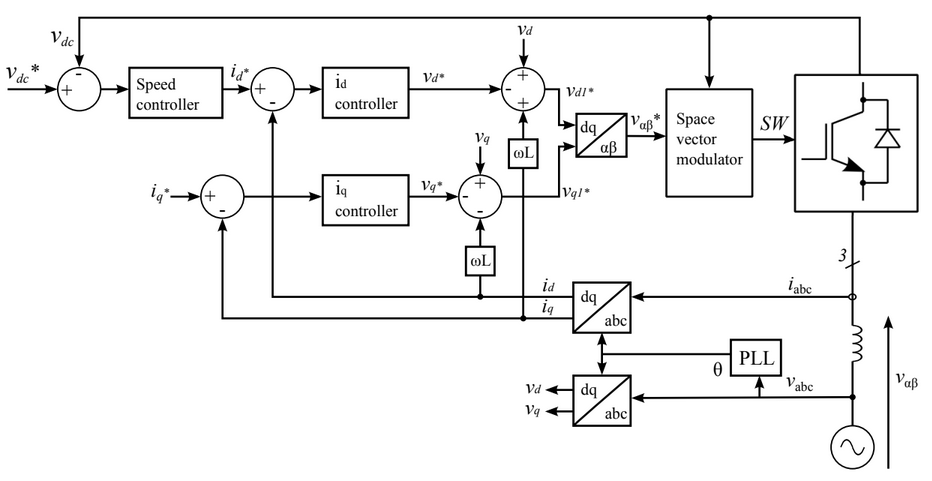
\includegraphics[width=0.8\textwidth]{./Figuras/controlepfc3ph.png}
	\legend{Fonte: \cite{3phPlecs}.}
	\label{fig:controlepfc3ph}
\end{figure}